\chapter{Propriétés des substances pures} 
\section{Substances pures}
Une \textbf{substance pure} est une substance de composition chimique 
homogène et stable, par exemple l'eau liquide ou un mélange eau/glace. 
Même si ce n'est pas le cas pour l'air, en l'absence de réaction 
chimique et de changement de phase, on peut le considérer comme telle 
: \textbf{substance pseudo-pure}.

\section{Équilibre des phases d'une substance pure}
Considérons de l'eau dans un cylindre contenu par un piston, le tout à 
20$^\circ$C. Si je chauffe l'eau, la pression exercée sera toujours la 
même. Tant qu'il reste une goutte d'eau, la température ne dépasse pas 
les 100$^\circ$C (pression et température constante), mais dès que 
celle-ci sera weg le gaz pourra se dilater et la température augmenter.\\

\noindent
\textbf{Attention !} Ceci illustre bien que durant un changement de 
phase, l'échange d'énergie n'est \textit{pas} lié à l'augmentation de 
la température ! Ce n'est pas parce que cela ne chauffe pas que de l'
énergie n'est pas dépensée : le changement de phase en consomme.

\begin{center}
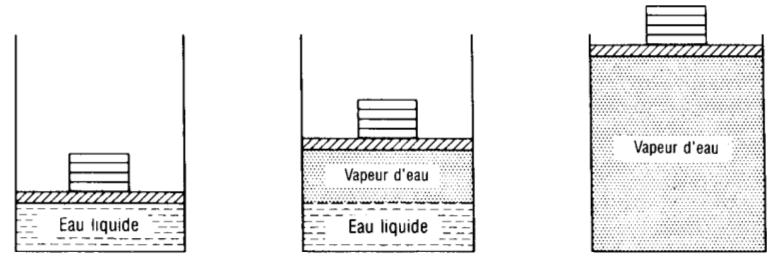
\includegraphics[scale=0.4]{ch3/image1}
\captionof{figure}{Si l'on fait varier la pression pour $T$, la 
pression de saturation est celle ou l'on passe de l'état liquide à 
vapeur (Spoil : loi de Clapeyron)}
\end{center}

On définit alors
\begin{description}
\item[Température de saturation] Température à laquelle la vaporisation 
se produit pour une pression donnée
\item[Pression de saturation] La même chose, mais pour une température 
donnée.
\item[Courbe de vaporisation] Relation fonctionnelle liant pression et 
température.
\end{description}


Tant que l'on parle de saturation, un \textbf{liquide saturé} est une 
substance à l'état liquide dans les contions $(p,T)$ de saturation. 
Une substance à l’état liquide à une température inférieure à la 
température de saturation à la pression donnée (et par conséquent à 
une pression supérieure à la pression de saturation à la température 
donnée) est appelée \textbf{liquide refroidi} ou \textbf{comprimé}.\\

\noindent
On peut également s'amuser à définir le \textbf{titre en vapeur} $
x = m_v/m$ où $m$ est la masse totale et $m_v$ la masse de vapeur. On 
parlera de \textbf{vapeur saturée} lorsqu'un état vapeur est dans les 
conditions de saturation et de \textbf{vapeur surchauffée} lorsque 
l'état vapeur est à température supérieure à la température de 
saturation.


\textit{Par exemple}, un liquide est saturé lorsqu'il bout. Au moment 
ou il est totalement évaporé, on sera en vapeur saturée.


\begin{center}
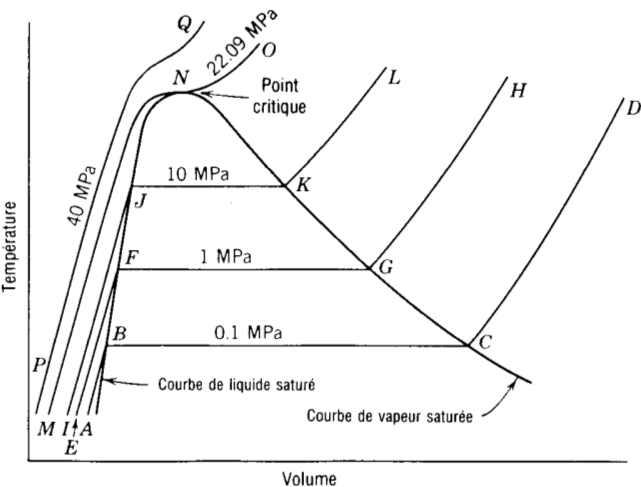
\includegraphics[scale=0.4]{ch3/image2}
\captionof{figure}{$AB$ : chauffage de l'eau, $BC$ : vaporisation, $CD$ : chauffage 
vapeur.}
\end{center}

Si l'on augmente la pression, on obtient la courbe $EFGH$. Pour une 
pression encore plus élevée, l'étape de vaporisation à température 
constante n'est plus (RIP) : $N$ est un point d'inflexion, c'est le 
\textbf{point critique}. Après la pression critique ($PQ$) l'
évolution de la température est continue et on ne peut plus 
dinstinguer la phase liquide de la phase vapeur. 

En partant de la glace à 0,26 kPa\footnote{Pour de la glace à 0.1 MPa, 
elle fond puis s'évapore pas de stress.}, la température s'élève jusqu'à 
-10$^\circ$C puis le liquide passe directement en vapeur : \textbf{
sublimation}. Le \textbf{point triple} marque le frontière entre 
les processus de fusion, d'évaporation et de sublimation.\\

\noindent
Notons qu'une substance peut exister sous plusieurs phases solides : 
un changement d'une telle phase à une autre est une transformation 
\textbf{allotropique}.

\section{Variables indépendantes d'une substance pure}
Une propriété des substances pures est que l'on peut décrire leur 
état à partir de \textbf{deux} variables indépendantes. Notons que
sur une courbe de changement de phase, $p$ et $T$ ne sont pas 
indépendants : on décrit un état saturé par $p,x$ ou $p,v$.


\section{Équation d'état pour la phase vapeur d'une substance pure}
On ne la présente plus (valable aux faibles masses volumiques) :
\begin{equation}
p\overline{v} = \overline{R}T
\end{equation}
où $\overline{R} = 8.314 \frac{kJ}{mole.K}$. En divisant cette 
équation par la masse molaire, on obtient la forme massique $pv = 
RT$ où $R = \overline{R}/M$.\\
A l'aide du facteur de compressibilité, on peut évaluer sa 
validité :
\begin{equation}
Z = \frac{p\overline{v}}{\overline{R}T}
\end{equation}
dont l'écart avec l'unité représente la dérivation entre le cas 
parfait et le réel.\\

\textsc{Exemple}. Pour l'azote :
\begin{itemize}
\item[$\bullet$] $Z \rightarrow 1$ si $p \rightarrow 0$.
\item[$\bullet$] Si $p = 4MPa$, $Z \searrow$ si $T \searrow$. Ceci 
est du au fait que les molécules sont assez proches pour que les 
forces d'attraction intermoléculaires prennent de l'importance.
\item[$\bullet$] Si $p > 30MPa$, la masse volumique est plus faible 
que celle donnée par la loi : les distances intermoléculaires sont 
si faible que les forces intermoléculaires sont répulsives.
\end{itemize}
\begin{center}
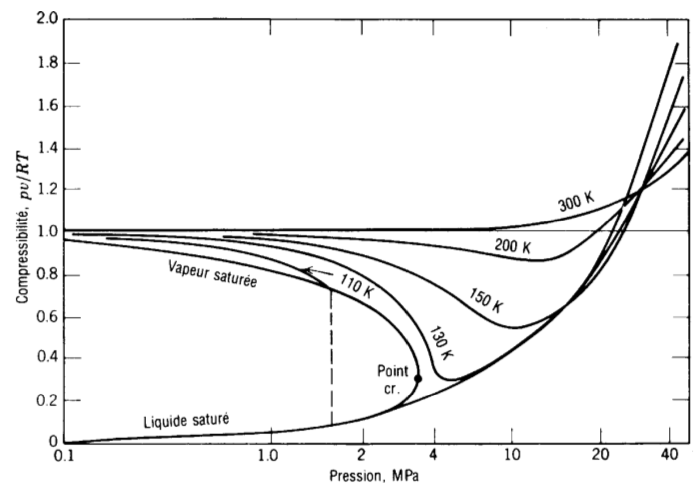
\includegraphics[scale=0.4]{ch3/image3}
\captionof{figure}{Compressibilité de l'azote}
\end{center}
Ce diagramme est valable pour tous les autres gaz : on le définit 
comme le \textit{diagramme de compressibilité généralisé}.\\

Comme tous les gaz ne sont pas comme moi, on a proposé plusieurs 
généralisations :
\begin{equation}
\begin{array}{ll}
\text{Van der Waals} & \left(p+\frac{a}{v^2}\right)(v-b) = RT \\
\text{Viriel} & Z = 1+\frac{B(T)}{v} + \frac{C(T)}{v^2} \\
\text{Redlich-Kwong} & p = \frac{RT}{v-b}-\frac{a}{\sqrt{T}v(v+b)}
\end{array}
\end{equation}


\section{Tables de variables thermodynamiques}
\textit{Voir séance d'exercices}


\section{Surfaces thermodynamiques}
Une substance pure se décrit avec deux variables, on peut le 
représenter en surface si l'on en ajoute une troisième (par 
exemple $p,v$ et $T$. Lorsqu'une seule phase est présente la 
surface est incurvée alors qu'elle est réglée lorsqu'il s'agit 
d'un mélange. Diverses courbes isothermes sont également 
représentée.

\begin{center}
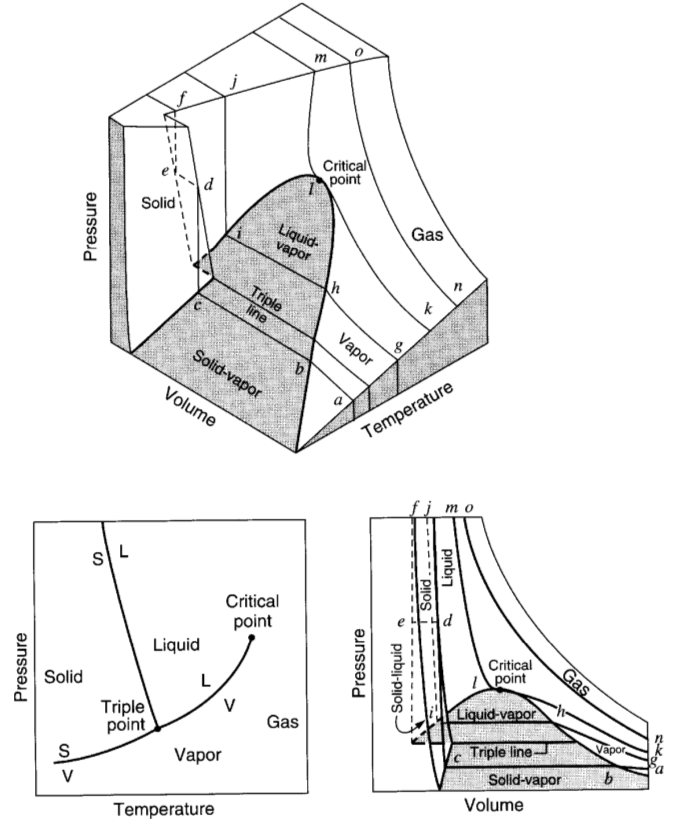
\includegraphics[scale=0.4]{ch3/image4}
\captionof{figure}{Surfaces thermodynamiques}
\end{center}








 



